\section{Discovered objects}

In 2017 the first interstellar object was discovered. Initially designated as
1I/2017 U1, this object is now commonly referred to as 1I/'Oumuamua.
Subsequently, in 2019, the discovery of the second interstellar object occurred.
Initially thought to be a comet, it was named C/2019 Q4. Upon confirming its
interstellar nature, this object became known as 2I/Borisov.

Despite originating from the same interstellar realm, both objects exhibited
distinct properties. These unique characteristics are thoroughly examined and
discussed in the subsequent subsections. For a more comprehensive analysis of
these objects and their attributes, reader is encouraged to refer to the work
by \cite{jewitt2022}.

\subsection{1I/'Oumuamua}

'Oumuamua was initially spotted on October 19, 2017, by the Pan-STARRS1
telescope in Hawaii. Initially designated as a comet under the identifier C/2017
U1, it was later reclassified as an asteroid. Figures \ref{fig:oumuamua_orbit},
\ref{fig:oumuamua_orbit_xz}, and \ref{fig:oumuamua_orbit_yz} show the orbit with
respect to the ecliptic of this interloper at the moment of its discovery from
different perspectives.

\begin{figure}[H]
  \centering
  \includegraphics[width=0.95\textwidth]{static/oumuamua/orbit_xy.png}
  \caption[Top view of the orbit of 1I/'Oumuamua through the solar system]{
    Top view of the orbit of 1I/'Oumuamua through the solar system at the time when it was
    discovered. The interloper presented a perihelion distance of 0.25 AU,
    closer than Mercury. 'Oumuamua exhibits a retrograde orbit moving
    towards the bottom of this figure.
  }
  \label{fig:oumuamua_orbit}
\end{figure}

\begin{figure}[H]
  \centering
  \includegraphics[width=0.95\textwidth]{static/oumuamua/orbit_xz.png}
  \caption[Front view of the orbit of 1I/'Oumuamua through the solar system]{
    Front view of the orbit of 1I/'Oumuamua through the solar system at the time when it was
    discovered. This perspective allows to visualize the high inclination of
    'Oumuamua as it passes through the solar system.}
  \label{fig:oumuamua_orbit_xz}
\end{figure}

\begin{figure}[H]
  \centering
  \includegraphics[width=0.95\textwidth]{static/oumuamua/orbit_yz.png}
  \caption[Side view of the orbit of 1I/'Oumuamua through the solar system]
  {
    Side view of the orbit of 1I/'Oumuamua through the solar system at the time when it was
    discovered. This perspective allows to visualize the retrograde motion of
    'Oumuamua as it passes through the solar system.
  }
  \label{fig:oumuamua_orbit_yz}
\end{figure}

'Oumuamua's orbit was calculated to be highly eccentric, with an eccentricity of
$1.20$, indicating a hyperbolic trajectory. Its velocity was estimated to be
approximately $26.0$ km/s. Upon entering the solar system, it approached from
the direction $\alpha_{\text{ICRS}},\; \delta_{\text{ICRS}} = 279^\circ.804,\;
  +33^\circ.997$, displaying an inclination significantly deviating from the solar
system's invariant plane and closely aligning with the solar apex, as discussed
in \cite{mamajek2017}. These characteristics collectively suggest an
interstellar origin, as elucidated in subsection
\ref{sec:expected_orbit_attributes}. Table \ref{tab:oumuamua_elements} provides
a summary of 'Oumuamua's orbit elements as of November 23, 2017.

\begin{table}[H]
  \centering
  \begin{tabular}{|c|c|}
    \hline
    Element                                    & Value                \\
    \hline
    Eccentricity ($e$)                         & 1.20                 \\
    Semi-major axis ($a$)                      & -1.27 au             \\
    Perihelion ($q$)                           & 0.26 au              \\
    Inclination ($i$)                          & 122.74 deg           \\
    Longitude of the ascending node ($\Omega$) & 24.59 deg            \\
    Argument of perihelion ($\omega$)          & 241.81 deg           \\
    Mean anomaly ($M$)                         & 51.16 deg            \\
    Mean motion ($n$)                          & 0.69 deg/d           \\
    Time of perihelion passage ($T_p$)         & 2017-Sep-09.50732138 \\
    \hline
  \end{tabular}
  \caption{Orbit elements of 1I/'Oumuamua as provided by the NASA SBDB.}
  \label{tab:oumuamua_elements}
\end{table}

Surprisingly, this first discovered ISO presented a non-gravitational
acceleration that could not be attributed to cometary properties. In addition,
observations could not determine jetting of particles, an effect experienced by
cometary objects.

'Oumuamua's shape was also a matter of debate. Due to its size, the interloper
appeared as a single point in all telescope images, like the one reproduced in
figure \ref{fig:oumuamua_shape}. At first, it was estimated to have a cigar-like
body. However, later studies solved the best fititng shape that matched the
observed lightcurves. The results indicate that 'Oumuamua should have a planar
disk shape, see \cite{seligman2022}.

\begin{figure}[H]
  \centering
  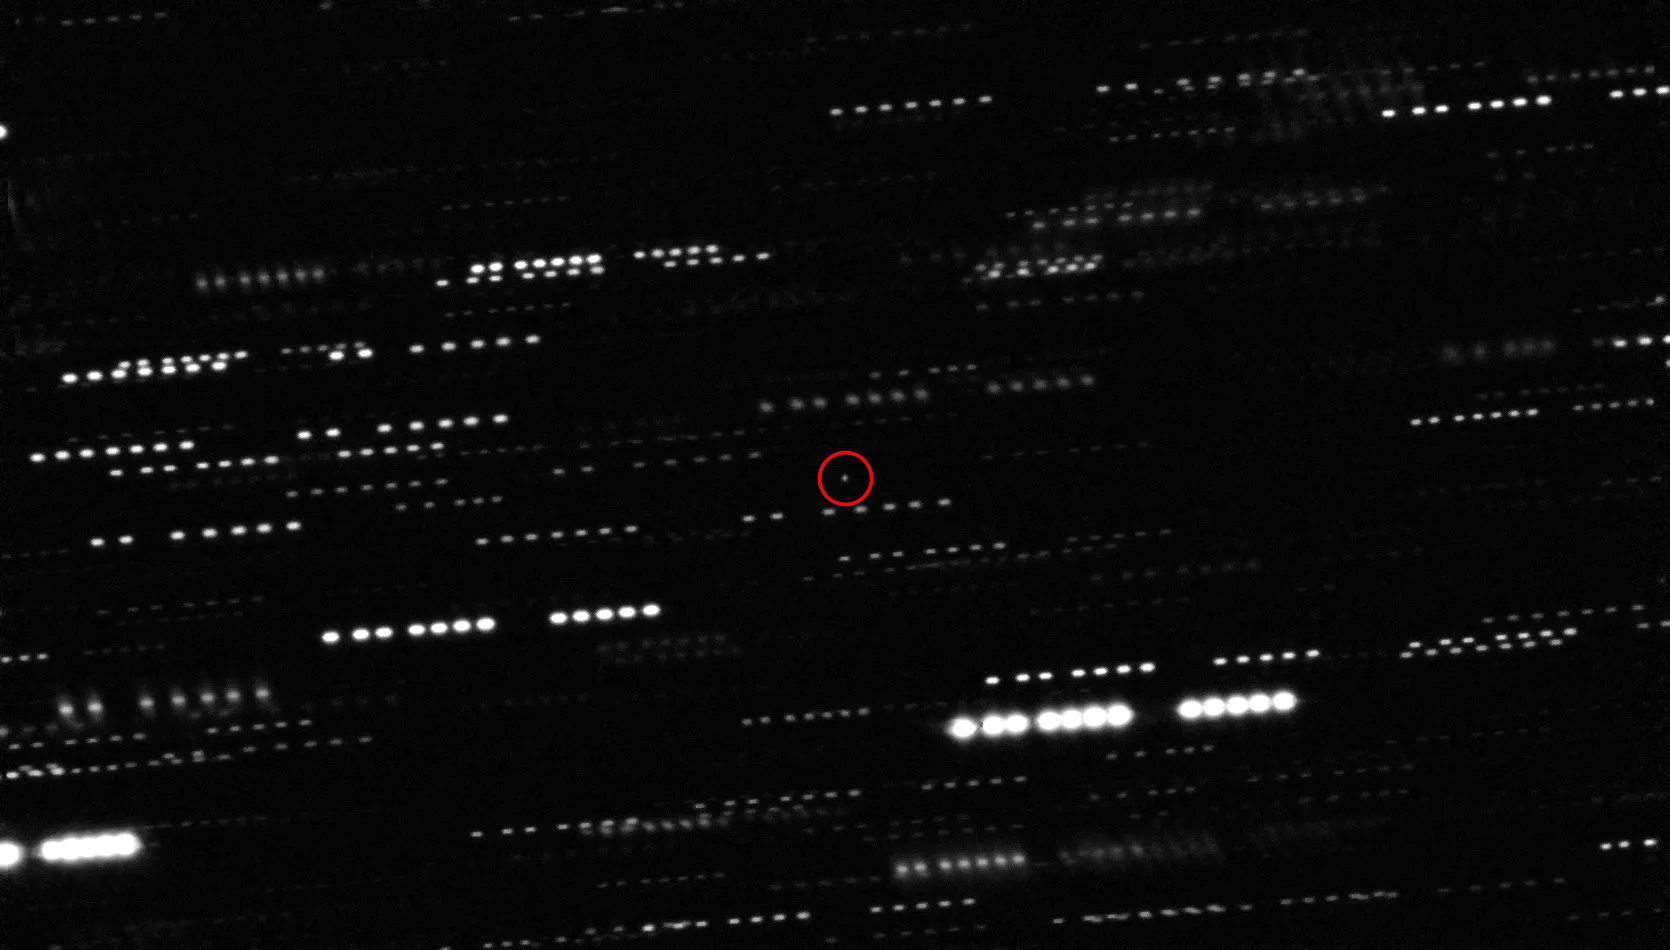
\includegraphics[width=0.95\textwidth]{static/oumuamua/shape.png}
  \caption['Oumuamua as seen by the ESO's VLT and GST telescopes]{
    1I/'Oumuamua as seen by the ESO's Very Large Telescope and the Gemini South
    Telescope. This image was released on September 9, 2023. It shows a
    combination of images taken by the two telecopes. The object is seen as
    a point in the center of the image. Background stars are seen as streaks
    due to the telescope's tracking of the object. No cometary tail or mass
    ejection is observed, raising questions about the non-gravitational
    acceleration presented by the interloper.
  }
  \label{fig:oumuamua_shape}
\end{figure}

Unfortunately, 'Oumuamua was discovered after its pasage through the perihelion
and could only be observed for about four weeks before becoming to faint. This
limited the amount of data that could be gathered about the object, increasing
the mistery about the first interstellar object.

\subsection{2I/Borisov}

Borisov was first sighted on August 30, 2019, by Gennady
Borisov\footnote{Borisov, an amateur astronomer from Crimea, detected the second
  interloper using his home-built 0.65 meters telescope.}. Initially labeled as a
comet bearing the identifier C/2019 Q4, it underwent reclassification as an
interstellar object subsequent to the determination of its remarkably high
eccentricity. Figure \ref{fig:borisov_orbit} shows the orbit of this interloper
at the moment of its discovery.

\begin{figure}[H]
  \centering
  \includegraphics[width=0.95\textwidth]{static/borisov/orbit_xy.png}
  \caption[Top view of the orbit of 2I/Borisov through the solar system]{
    Top view of the orbit of 2I/Borisov through the solar system. Its eccentricity is
    close to 3.36, making it the most eccentric object observed up to date
    and discarding the possibility of being gravitationally bounded to the Sun.
    Borisov presented a perihelion distance of 2.01 AU, closer than Mars.
  }
  \label{fig:borisov_orbit}
\end{figure}


\begin{figure}[H]
  \centering
  \includegraphics[width=0.95\textwidth]{static/borisov/orbit_xz.png}
  \caption[Front view of the orbit of 2I/Borisov through the solar system]{
    Front view of the orbit of 2I/Borisov through the solar system. Despite the
    apparent close distance with the Martian planet, this view shows that both
    celestial objects were actually far from each other.}
  \label{fig:borisov_orbit_xz}
\end{figure}

\begin{figure}[H]
  \centering
  \includegraphics[width=0.95\textwidth]{static/borisov/orbit_yz.png}
  \caption[Side view of the orbit of 2I/Borisov through the solar system]{
    Side view of the orbit of 2I/Borisov through the solar system. Even if this
    view suggests that Borisov could have a high inclination, the value for this
    parameter was not as high as the one for the first discovered interloper.}
  \label{fig:borisov_orbit_yz}
\end{figure}

With an eccentricity of $3.36$ and a velocity of $32.2$ km/s, Borisov exhibited
a hyperbolic orbit. Its inclination of $44.1$ degrees incoming from
constellation Cassiopeia further confirmed its ISO nature. Table
\ref{tab:borisov_elements} provides a summary of Borisov's orbit elements as of
August 1, 2020.

\begin{table}[H]
  \centering
  \begin{tabular}{|c|c|}
    \hline
    Element                                    & Value                \\
    \hline
    Epoch ($t$)                                & August 1, 2020       \\
    Eccentricity ($e$)                         & 3.36                 \\
    Semi-major axis ($a$)                      & -0.85 au             \\
    Perihelion ($q$)                           & 2.01 au              \\
    Inclination ($i$)                          & 44.05 deg            \\
    Longitude of the ascending node ($\Omega$) & 308.15 deg           \\
    Argument of perihelion ($\omega$)          & 209.12 deg           \\
    Mean anomaly ($M$)                         & 296.54 deg           \\
    Mean motion ($n$)                          & 1.25 deg/d           \\
    Time of perihelion passage ($T_p$)         & 2019-Dec-08.54507021 \\
    \hline
  \end{tabular}
  \caption{Orbit elements of 2I/Borisov as provided by the NASA SBDB.}
  \label{tab:borisov_elements}
\end{table}

Unlike 'Oumuamua, Borisov displayed a cometary tail. Remarkably, the NASA/ESA
Hubble Space Telescope captured images of this interloper, as depicted in figure
\ref{fig:borisov_shape}.

Analysis revealed that the coma of 2I/Borisov contained significantly more
carbon monoxide (CO) gas than water (H2O), with abundances exceeding 173\%,
surpassing typical cometary compositions within our solar system by over
threefold. Additionally, hydrogen cyanide (HCN) was also detected in the gas
expelled by the comet, with levels comparable to those observed in other solar
system comets \cite{bodewits2020}.

\begin{figure}[H]
  \centering
  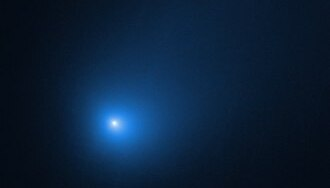
\includegraphics[width=0.95\textwidth]{static/borisov/shape.jpg}
  \caption[Borisov as seen by the NASA/ESA Hubble Space Telescope]{
    2I/Borisov as seen by the NASA/ESA Hubble Space Telescope. This image was
    released on December 12, 2019, when the interloper was close to the Sun. Its
    cometary properties are evident in this image. Borisov's tail is seen as a
    faint streak extending from the object. It is believed that the tail is composed
    of
  }
  \label{fig:borisov_shape}
\end{figure}

\subsection{Other interstellar candidates}

The interest in interstellar objects has lead a research on previously
discovered objects, in particular interstellar meteors (IM). Interstellar
meteors are meter-scale objects that collide with Earth from a trajectory that
is gravitationally unbound to the Sun, meaning they originate from outside our
solar system.

Two confirmed interstellar meteors have been identified so far:

\begin{itemize}
  \item CNEOS 2014-01-08 (also known as IM1 or the Manus Island fireball), which
        was detected in 2014 and confirmed as interstellar in 2022 by the U.S. Space
        Command.
  \item CNEOS 2017-03-09 (also known as IM2), which was discovered in 2022 and is
        estimated to have been 10 times more massive than IM1, around 1 meter in
        size.
\end{itemize}

Both IM1 and IM2 were moving at extremely high speeds relative to the local
standard of rest - IM1 at 60 km/s and IM2 at 40 km/s. This high velocity is a
key indicator of their interstellar origin. Analysis of the meteors' material
strength suggests they were tougher than typical iron meteorites, implying they
may not have originated from a planetary system like our own. Plans are underway
to try and retrieve fragments of these interstellar meteors for further study,
which could provide important insights into their composition and origins, see
\cite{siraj2022discovery}.
